\documentclass[tikz,border=10pt]{standalone}
\begin{document}
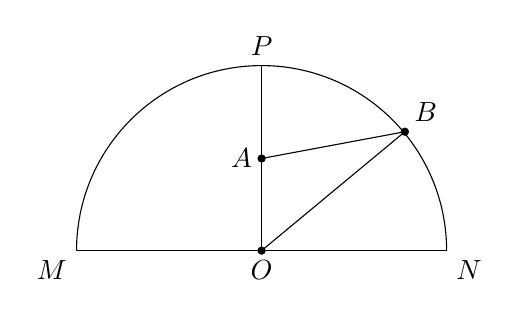
\begin{tikzpicture}
\coordinate (M) at (-2.35,0);
\coordinate (O) at (0,0);
\coordinate (N) at (2.35,0);
\coordinate (P) at (0,2.35);
\coordinate (A) at (0,1.17);
\coordinate (B) at (1.82,1.51);

\draw (M) -- (N);
\draw (N) arc (0:180:2.35);
\draw (P) -- (O);
\draw (A) -- (B);
\draw (O) -- (B);

\fill (O) circle (1.5pt);
\fill (A) circle (1.5pt);
\fill (B) circle (1.5pt);

\node[above] at (P) {$P$};
\node[left] at (A) {$A$};
\node[above right] at (B) {$B$};
\node[below left] at (M) {$M$};
\node[below] at (O) {$O$};
\node[below right] at (N) {$N$};
\end{tikzpicture}
\end{document}
